\section{Forward Tracking System}
\label{overview}

The CLAS12 Forward Detector is constructed around a toroidal magnet consisting of six 
iron-free superconducting coils.  The particle detection system consists of drift 
chambers to determine charged-particle trajectories, Cherenkov detectors 
for electron/pion separation, scintillation counters for flight-time 
measurements, and calorimeters to identify electrons and high-energy neutral 
particles.  An overview of the CLAS12 subsystems and geometry may be found in the 
CLAS12 overview paper~\cite{clas12-nim} in this volume.  A schematic view of the 
torus magnet with drift chambers
attached is shown in Fig.~\ref{chambers-and-torus}.   The drift chambers are 
triangular boxes attached to the magnet cryostat.  
This assembly of the magnet and chambers is referred to as the ``Forward Tracker''. 

The Forward Tracker can detect charged particles emerging from the target with
momenta greater than 200~MeV at polar angles from roughly 5$^{\circ}$ to 
40$^{\circ}$.  Particles with lower momentum are swept out of the tracking
volume by the torus magnetic field.  
Because the coils of the torus magnet represent a ``dead area''
in which we cannot detect charged particles, we designed the chamber endplates
and attached electronics to be as thin as possible.  The resulting azimuthal
coverage varies from 50\% of 2$\pi$ at 5$^{\circ}$ to 80\% of 2$\pi$ at 40$^{\circ}$.

%%%%%%%%%%%%%%%%%%%%%% Figure : CLAS 3D Picture %%%%%%%%%%%%%%%%%%%%%%%%%%
\begin{figure}[htbp]
\vspace{5.5cm}
\begin{picture}(50,50)
\put(2,0)
{\hbox{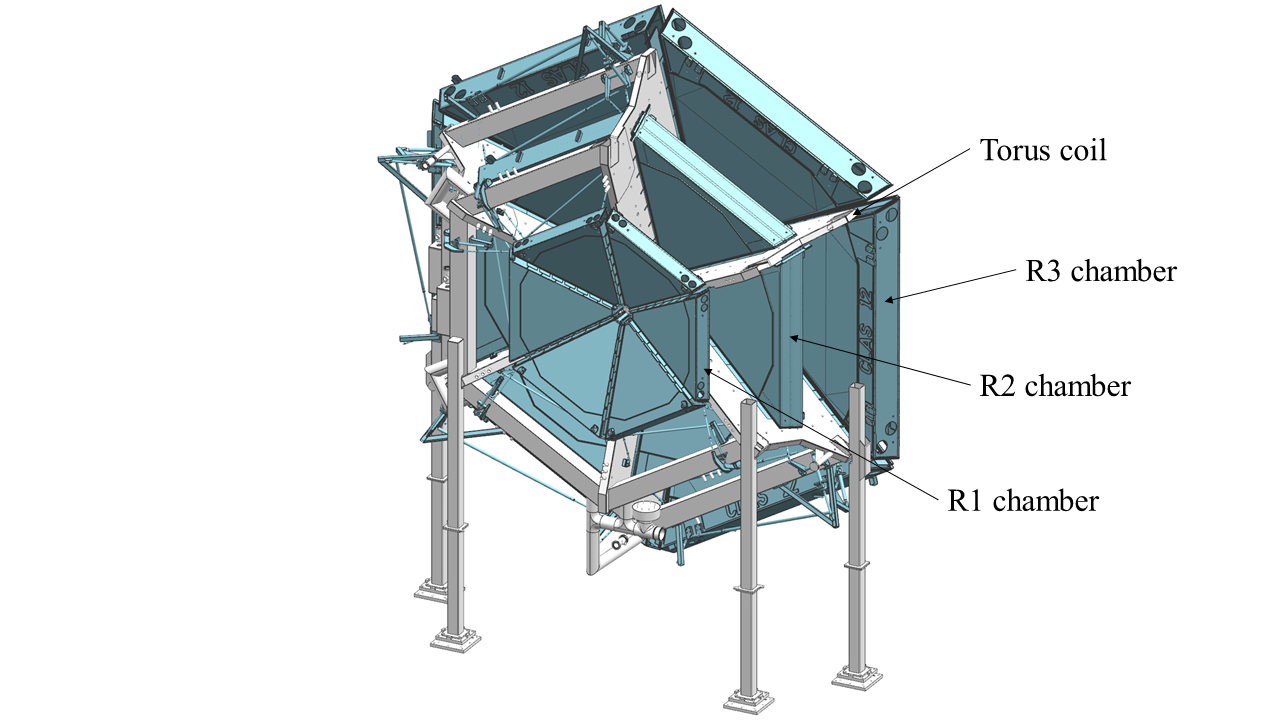
\includegraphics[width=0.6\textwidth,natwidth=610,natheight=642]{img/chambers-and-torus.png}}}
\end{picture}
\caption{\small{A model drawing of the torus magnet (light gray) with drift chambers (darker blue) attached.
Note that the cable runs and gas lines have been removed for clarity.  The largest
chambers are approximately equilateral triangular solids with 4~m long sides and 0.8~m depth.}}
\label{chambers-and-torus}
\end{figure}
%%%%%%%%%%%%%%%%%%%%%%%%%%%%%%%%%%%%%%%%%%%%%%%%%%%%%%%%%%%%%%%




















































